19. По теореме Виета $x_1+x_2=\cfrac{a}{2},\ x_1x_2=-\cfrac{a}{2}.$ Тогда $\cfrac{x_1}{x_2}+\cfrac{x_2}{x_1}=\cfrac{x_1^2+x_2^2}{x_1x_2}=\cfrac{(x_1+x_2)^2-2x_1x_2}{x_1x_2}=\cfrac{\cfrac{a^2}{4}+a}{-\cfrac{a}{2}}=-\cfrac{a+4}{2}=-3,5\Rightarrow a=3.$ Построим параболу $y=2x^2-3x-3$ по трём точкам \\ $(-2;11),\ \left(\cfrac{7}{2};11
ight),\ \left(\cfrac{3}{4};-\cfrac{33}{8}
ight).$
$$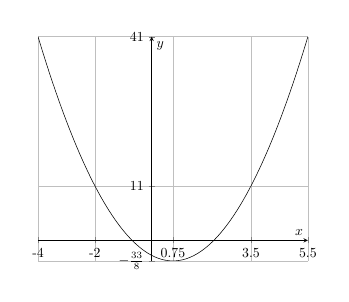
\begin{tikzpicture}[scale=0.5]
\begin{axis}[
    axis lines = middle,
    grid=major,
    legend pos={south west},
    xlabel = {$x$},
    ylabel = {$y$},
    %ymin=-80,
    %ymax=250,
    xtick={-4, -2, 0.75, 3.5, 5.5},
    xticklabels={-4, -2, 0.75, 3.5, 5.5},
    ytick={41,11,-4.125},
    yticklabels={41,11,$-\frac{33}{8}$}             ]
	\addplot[domain=-4:5.5, samples=100, color=black] {2*x*x-3*x-3};
%\addplot[domain=-3.1:2.5, samples=100, color=red] {70*abs(1-2*abs(abs(x)-2))-10*x^2+10*x-70};
	%\addlegendentry{$\text{Рис. 1}$};
\end{axis}
\end{tikzpicture}$$
